\documentclass[conference]{IEEEtran}
\IEEEoverridecommandlockouts
\usepackage[T1]{fontenc}
\usepackage[utf8]{inputenc}
\usepackage{amsmath,amssymb,booktabs,graphicx,cite,url,balance,flushend}
\renewcommand{\topfraction}{0.92}
\renewcommand{\dbltopfraction}{0.92}
\renewcommand{\textfraction}{0.06}
\renewcommand{\floatpagefraction}{0.75}
\renewcommand{\dblfloatpagefraction}{0.75}
\setcounter{topnumber}{4}
\setcounter{dbltopnumber}{4}
\setcounter{totalnumber}{6}
\pdfinfo{
  /Title (Disentangling Obstacle Information and APF Guidance in Hybrid A2C-APF UAV Navigation under Wind)
  /Author (Hieu Ta Chi; Huy Nguyen Anh; Hoa Vu Minh)
  /Subject (Component and information ablations for hybrid A2C-APF UAV guidance)
  /Keywords (UAV navigation, reinforcement learning, A2C, artificial potential field, ablation, trajectory variation)
}

\title{Disentangling Obstacle Information and APF Guidance in Hybrid A2C--APF UAV Navigation under Wind}
\author{\IEEEauthorblockN{Hieu Ta Chi\textsuperscript{1}, Huy Nguyen Anh\textsuperscript{2}, Hoa Vu Minh\textsuperscript{3}}
\IEEEauthorblockA{\textsuperscript{1,2}Thuyloi University, Hanoi, Viet Nam\\
\textsuperscript{3}Faculty of International Business, Foreign Trade University, Hanoi, Viet Nam\\
\textsuperscript{1}hieutc@tlu.edu.vn, \textsuperscript{2}huyabcd2004@gmail.com, \textsuperscript{3}k62.2312550029@ftu.edu.vn}}

\begin{document}
\maketitle

\begin{abstract}
Hybrid reinforcement-learning and reactive guidance controllers for cluttered UAV navigation confound two
distinct ingredients: the analytical guidance law and the obstacle information that law consumes. We disentangle
them in a wind-perturbed point-mass simulator by adding a geometry-aware A2C baseline (H3) whose 68-dimensional
observation carries padded raw AABB geometry but no potential-field computation, alongside the hybrid (H0),
obstacle-blind A2C (H1), and APF-only (H2) configurations. All learned configurations use four 300-m maps,
five independently trained 5M-step runs per map, and a corrected schedule of 50 unique evaluation seeds per run
(the prior 50-slot schedule contained only 32 distinct seeds). With corrected seeds, H0 completes 1000/1000
rollouts versus 938 for H3 and 848 for H1. The 15.2-percentage-point H0--H1 reliability gap decomposes into
$+9.0$ points associated with obstacle information (H3$-$H1, $p=0.250$) and $+6.2$ points associated with the
analytical channel (H0$-$H3, $p=0.125$); neither component is individually significant at $n=20$ paired units.
In contrast, sampled trajectory variation separates cleanly: H0$-$H3 jitter and acceleration differences are
large and significant ($d_z=-1.97$ and $-4.08$, $p<0.001$) while H3$-$H1 is null ($p\approx0.90$). A frozen-policy
wind sweep shows graceful degradation to twice the training intensity (H0: 98.6\% at $2\times$), a predeclared
APF sensitivity grid shows that H2's earlier 5.5\% success measured a dead center-distance repulsion term
(surface-distance APF removes all collisions but still times out in 56\% of episodes), and held-out layouts
transfer for three of four families while one unseen family collapses all controllers. We report all null
results and label every claim with the evidence level that supports it.
\end{abstract}

\begin{IEEEkeywords}
UAV navigation, deep reinforcement learning, A2C--APF guidance, ablation, information matching, trajectory variation.
\end{IEEEkeywords}

\section{Introduction}
Low-altitude navigation in clutter demands sustained goal progress, collision avoidance, and control that does
not vary abruptly under disturbance. Artificial potential fields (APF) supply cheap reactive guidance but suffer
local minima, oscillation, and gain sensitivity \cite{khatib1986real}; sampling-based planners address known-map
routing under a different information structure \cite{lavalle1998rrt,karaman2011sampling}; reinforcement learning
(RL) learns a state-to-action map whose reliability depends on seeds, rewards, observations, and termination
logic \cite{henderson2018deep,dulac2021challenges}. Coupling APF with RL is therefore plausible but not novel
\cite{jin2025hybrid,xiao2025vapf,lee2025apfppo}, which moves the scientific question from architecture to
attribution: \emph{how much of a hybrid controller's measured reliability is associated with the obstacle
information its analytical channel consumes, and what incremental evidence remains for the analytical guidance
itself under wind disturbance?}

Our prior submission evaluated H0 (hybrid) against H1 (A2C-only) and H2 (APF-only) and already stated the core
threat: because the learned observation contains no obstacle geometry, H0--H1 measures the APF channel
\emph{together with} its privileged geometric input. Reviewers correctly identified this confound as the central
weakness, together with a questionable APF-only baseline, fixed-map ceiling effects, and an evaluation-seed
schedule with duplicate seeds. This revision answers each point with new experiments rather than rewording:
a matched-information baseline, a corrected seed schedule, a frozen-policy wind stress test, a predeclared APF
sensitivity grid, held-out layouts, action-component logging, and an evaluation-time blend sensitivity study.

Contributions: (i) a geometry-aware A2C configuration (H3) with a deterministic padded raw-geometry observation
and no potential-field term, trained at the same 5M-step budget; (ii) a corrected 50-unique-seed evaluation
protocol with paired inference at the (map, training-run) unit; (iii) an additive decomposition of the
hybrid--blind reliability gap into an information component and an analytical-channel component, with explicit
significance levels; (iv) frozen-policy wind and held-out stress tests plus a full APF distance-basis/$d_0$
sensitivity grid, all reported in full; (v) a complete machine-readable result ledger and analysis scripts.
We claim no new algorithm, no ranking against PPO/SAC/RRT, no physical-flight readiness, and no generalization.

\section{Related Work}
\subsection{Reactive and sampling-based navigation}
APF computes local attraction and repulsion online \cite{khatib1986real}; RRT and asymptotically optimal variants
plan globally when the map is known \cite{lavalle1998rrt,karaman2011sampling}. Recent hybrid planners and UAV
reviews trade off global search, online response, and computation \cite{zheng2025uav,li2024gapf}, but are not
directly comparable to a wind-perturbed feedback controller without matched sensing and replanning assumptions.
\subsection{Actor--critic control and empirical rigor}
A2C uses a critic to reduce policy-gradient variance \cite{mnih2016a3c}; PPO, SAC, and DDPG are important
continuous-control alternatives \cite{schulman2017ppo,haarnoja2018sac,lillicrap2016ddpg}. Deep-RL outcomes vary
substantially with implementation choices \cite{henderson2018deep}, and sim-to-real transfer adds safety and
perception challenges \cite{dulac2021challenges,tobin2017domain}. We therefore treat A2C as a compact on-policy
reference that makes component attribution tractable, not as a state-of-the-art claim.
\subsection{Hybrid APF--RL and wind-aware control}
Potential guidance may shape rewards, constrain actions, or blend with policy output
\cite{jin2025hybrid,xiao2025vapf,lee2025apfppo}; wind-aware tracking and disturbance adaptation form a parallel
line \cite{wu2024wind,neuralfly2022,datt2021,mellinger2011minimum}. Our design uses direct convex action blending
and asks what each ingredient contributes, extending the information-matching critique that applies to all
hybrid evaluations whose learned observation lacks geometry.

\section{Controller, Observations, and Simulator}
\subsection{Shared dynamics, reward, and termination}
The episodic MDP uses $\gamma=0.99$, point-mass dynamics with $m=0.5$ kg, $k_d=0.12$, $g_0=9.81$ m/s$^2$,
$\Delta t=0.1$ s, per-axis force limit 12 N, semi-implicit Euler integration, altitude clamp $z\in[5,6]$ m with
vertical-velocity reset, and wind as air velocity inside the linear drag term:
\begin{align}
F_t &= 12\,\mathrm{clip}(u_t,-1,1) - m g_0 e_z,\\
a_t &= (F_t - k_d (v_t - w_t))/m .
\end{align}
Obstacles are axis-aligned boxes; collision uses a swept slab test with zero vehicle inflation and has priority
over success; success requires final goal distance below 3 m. The horizon is
$H=\lfloor(\|g_{xy}-p_{0,xy}\|/(v_{\rm ref}\Delta t))\,1.8\rfloor+300=1507$ transitions for the 300-m maps.
The reward combines progress shaping $3(d_{t-1}-d_t)$, step cost $-0.05$, collision $-200$, success bonus
$\max(80,150(1-n_t/H))$, a clearance band term $0.3(\delta_t-2)$ for $2<\delta_t<8$ m using signed
nearest-surface distance, and an altitude term that is inactive after clamping (reported as dead code).
\subsection{Observations and the matched-information baseline}
H0 and H1 use the 12-dimensional observation $s_t=[p_t, v_t, g-p_t, w_t]\in\mathbb{R}^{12}$ with no obstacle term.
H3 appends a deterministic padded geometry block: the $K=8$ nearest obstacles sorted by distance to the vehicle,
each contributing relative center divided by 300 m (3), half-extents divided by 300 m (3), and a validity mask
(1), zero-padded when fewer than $K$ obstacles exist; the observation is therefore 68-dimensional and contains
raw geometry only---never an APF force. $K=8$ covers every layout produced by the map generator
(random and mixed: 6 boxes; corridor: 8; barrier: 2). H3 executes the pure learned action: no APF force is
computed into the command and no blending is applied.
\subsection{APF channel and its two distance bases}
The attractive term is $F_{\rm att}=k_{\rm att}\,q_t/(\|q_t\|+\epsilon)$ with $k_{\rm att}=0.04$. The repulsive
term uses gain $k_{\rm rep}=18$ and influence radius $d_0$ inside a normalized-then-clipped sum. Two distance
bases are studied: the shipped \emph{center} basis $d_i=\|p_t-c_i\|+\epsilon$, and a \emph{surface} basis using
signed nearest-surface distance with the push direction away from the nearest surface point. The hybrid command
is $u_t=(1-\lambda_t)a_t^{\rm A2C}+\lambda_t a_t^{\rm APF}$ with
$\lambda_t=\mathrm{clip}(1-\|g-p_t\|/300,\,0.15,\,0.55)$; fixed-$\lambda$ variants are evaluated only as
deployment-time sensitivity, since policies are trained under the adaptive schedule.
\subsection{Wind and its stress-test scaling}
Wind is a vector AR(1) gust ($\tau=0.9$ s, stationary gust std 1.2 m/s horizontal, 0.36 m/s vertical, horizontal
cross-correlation 0.35) added to a 2 m/s base with uniform random direction per episode. The stress test applies
one interpretable rule: the entire wind velocity vector is multiplied by $\texttt{wind\_scale}\in\{0,0.5,1,1.5,2\}$
at every step; scale 1.0 reproduces the training setting exactly.

\section{Experimental Protocol}
\subsection{Configurations}
Table~\ref{tab:matrix} makes the information structure explicit. H4 (same-grid spline resampling) is removed as
a named configuration; it altered no action, outcome, or same-grid variation value and survives only as this note.
\begin{table}[t]
\centering
\caption{Controller matrix. ``Geo to policy'' is the learned observation; ``Geo to APF'' is the analytical channel.}
\label{tab:matrix}
\resizebox{\columnwidth}{!}{%
\begin{tabular}{llccccc}
\toprule
Config & Learned? & Geo to policy & Geo to APF & APF action & Adaptive blend & Budget\\
\midrule
H0 hybrid & A2C & no & centers & yes & yes & 5M/unit\\
H1 blind  & A2C & no & no & no & no & 5M/unit\\
H2 APF    & no  & n/a & grid & yes & n/a & 0\\
H3 geo    & A2C & yes (68-D) & no & no & no & 5M/unit\\
\bottomrule
\end{tabular}}
\end{table}
\subsection{Maps, seeds, and inference units}
Four training maps (random, corridor, barrier, mixed; 300 m, density 0.8) and four held-out maps generated with
new seeds (7101/7113/7119/7127) under the same generator. Learned configurations use training seeds
101/211/307/401/503 with 5,000,000 environment steps per (map, seed) unit, one environment, CPU, lr $3\times10^{-4}$,
$n_{\rm steps}=256$, GAE $\lambda=0.95$, entropy 0.02, gradient norm 0.5; H3 additionally seeds PyTorch through
the library seed setter. Evaluation uses deterministic actions and the corrected schedule
$\texttt{seed}=\texttt{base}+\texttt{episode}$ with bases $\{2001,2011,2021,2031,2041\}$ and episodes 0--9,
i.e.\ 50 \emph{unique} seeds per unit shared across configurations and wind scales (the prior schedule collapsed
to 32 distinct seeds with 18 exact repeats per unit). Inference uses paired two-sided Wilcoxon signed-rank tests
and Cohen's $d_z$ on the 20 (map, training-run) units; rollout proportions carry descriptive Wilson intervals
only; $p$-values are exploratory and uncorrected, reported with exact values and effect sizes. Held-out
evaluation gives H0 and H3 the new geometry through their respective channels and is therefore controller-level
transfer with map geometry available, not obstacle-free zero-shot generalization. The APF grid
(basis $\times\ d_0\in\{4,6,8,12\}$ m) was fixed before any result was inspected, and all eight settings are reported.

\section{Results}
\subsection{Corrected-seed component comparison}
Table~\ref{tab:outcomes} gives rollout accounting on the training maps. H0 completes every rollout; H3 loses
62 rollouts, all to collision (zero timeouts); H1 loses 152, split into 45 collisions and 107 timeouts.
\begin{table}[t]
\centering
\caption{Corrected-seed outcomes on training maps (1000 rollouts per configuration).}
\label{tab:outcomes}
\resizebox{\columnwidth}{!}{%
\begin{tabular}{lccccc}
\toprule
Config & Success & SR (Wilson 95\%) & Coll. & Timeout & Eff.\ (success only)\\
\midrule
H0 & 1000 & 1.000 (0.996--1.000) & 0 & 0 & $0.883\pm0.075$\\
H3 & 938 & 0.938 (0.921--0.952) & 62 & 0 & $0.886\pm0.086$\\
H1 & 848 & 0.848 (0.824--0.870) & 45 & 107 & $0.894\pm0.098$\\
\bottomrule
\end{tabular}}
\end{table}
Paired unit-level contrasts (Table~\ref{tab:paired}) show the reliability ordering H0 $>$ H3 $>$ H1 with a
significant total gap (H0$-$H1 $+0.152$, $d_z=0.491$, $p=0.0156$) but non-significant components
(H3$-$H1 $+0.090$, $p=0.250$; H0$-$H3 $+0.062$, $p=0.125$). Trajectory variation behaves oppositely:
H0$-$H3 jitter and acceleration differences are large and significant ($d_z=-1.97$, $-4.08$; $p<0.001$) while
H3$-$H1 is null ($d_z=-0.07$, $+0.27$; $p\approx0.90$). Efficiency, clearance, and step-count differences between
H0 and H1 remain unsupported ($p=0.768$, $0.927$, $0.143$); H0 uses more steps than H3 ($+26.9$, $d_z=1.37$,
$p<0.001$), i.e.\ the hybrid trades speed for completion.
\begin{table}[t]
\centering
\caption{Paired unit-level contrasts (20 units; efficiency 19--20). Diffs are row-config minus column-config.}
\label{tab:paired}
\resizebox{\columnwidth}{!}{%
\begin{tabular}{lccc}
\toprule
Contrast / metric & diff & $d_z$ & $p$\\
\midrule
H0$-$H1 success & $+0.152$ & 0.491 & 0.0156\\
H3$-$H1 success & $+0.090$ & 0.276 & 0.250\\
H0$-$H3 success & $+0.062$ & 0.410 & 0.125\\
H0$-$H1 jitter & $-27.24$ & $-1.75$ & $<0.001$\\
H3$-$H1 jitter & $-1.13$ & $-0.07$ & 0.898\\
H0$-$H3 jitter & $-26.11$ & $-1.97$ & $<0.001$\\
H0$-$H3 acceleration & $-8.87$ & $-4.08$ & $<0.001$\\
H0$-$H1 efficiency & $-0.006$ & $-0.06$ & 0.768\\
H0$-$H1 clearance & $-0.563$ & $-0.07$ & 0.927\\
\bottomrule
\end{tabular}}
\end{table}
\begin{figure*}[!t]
\centering
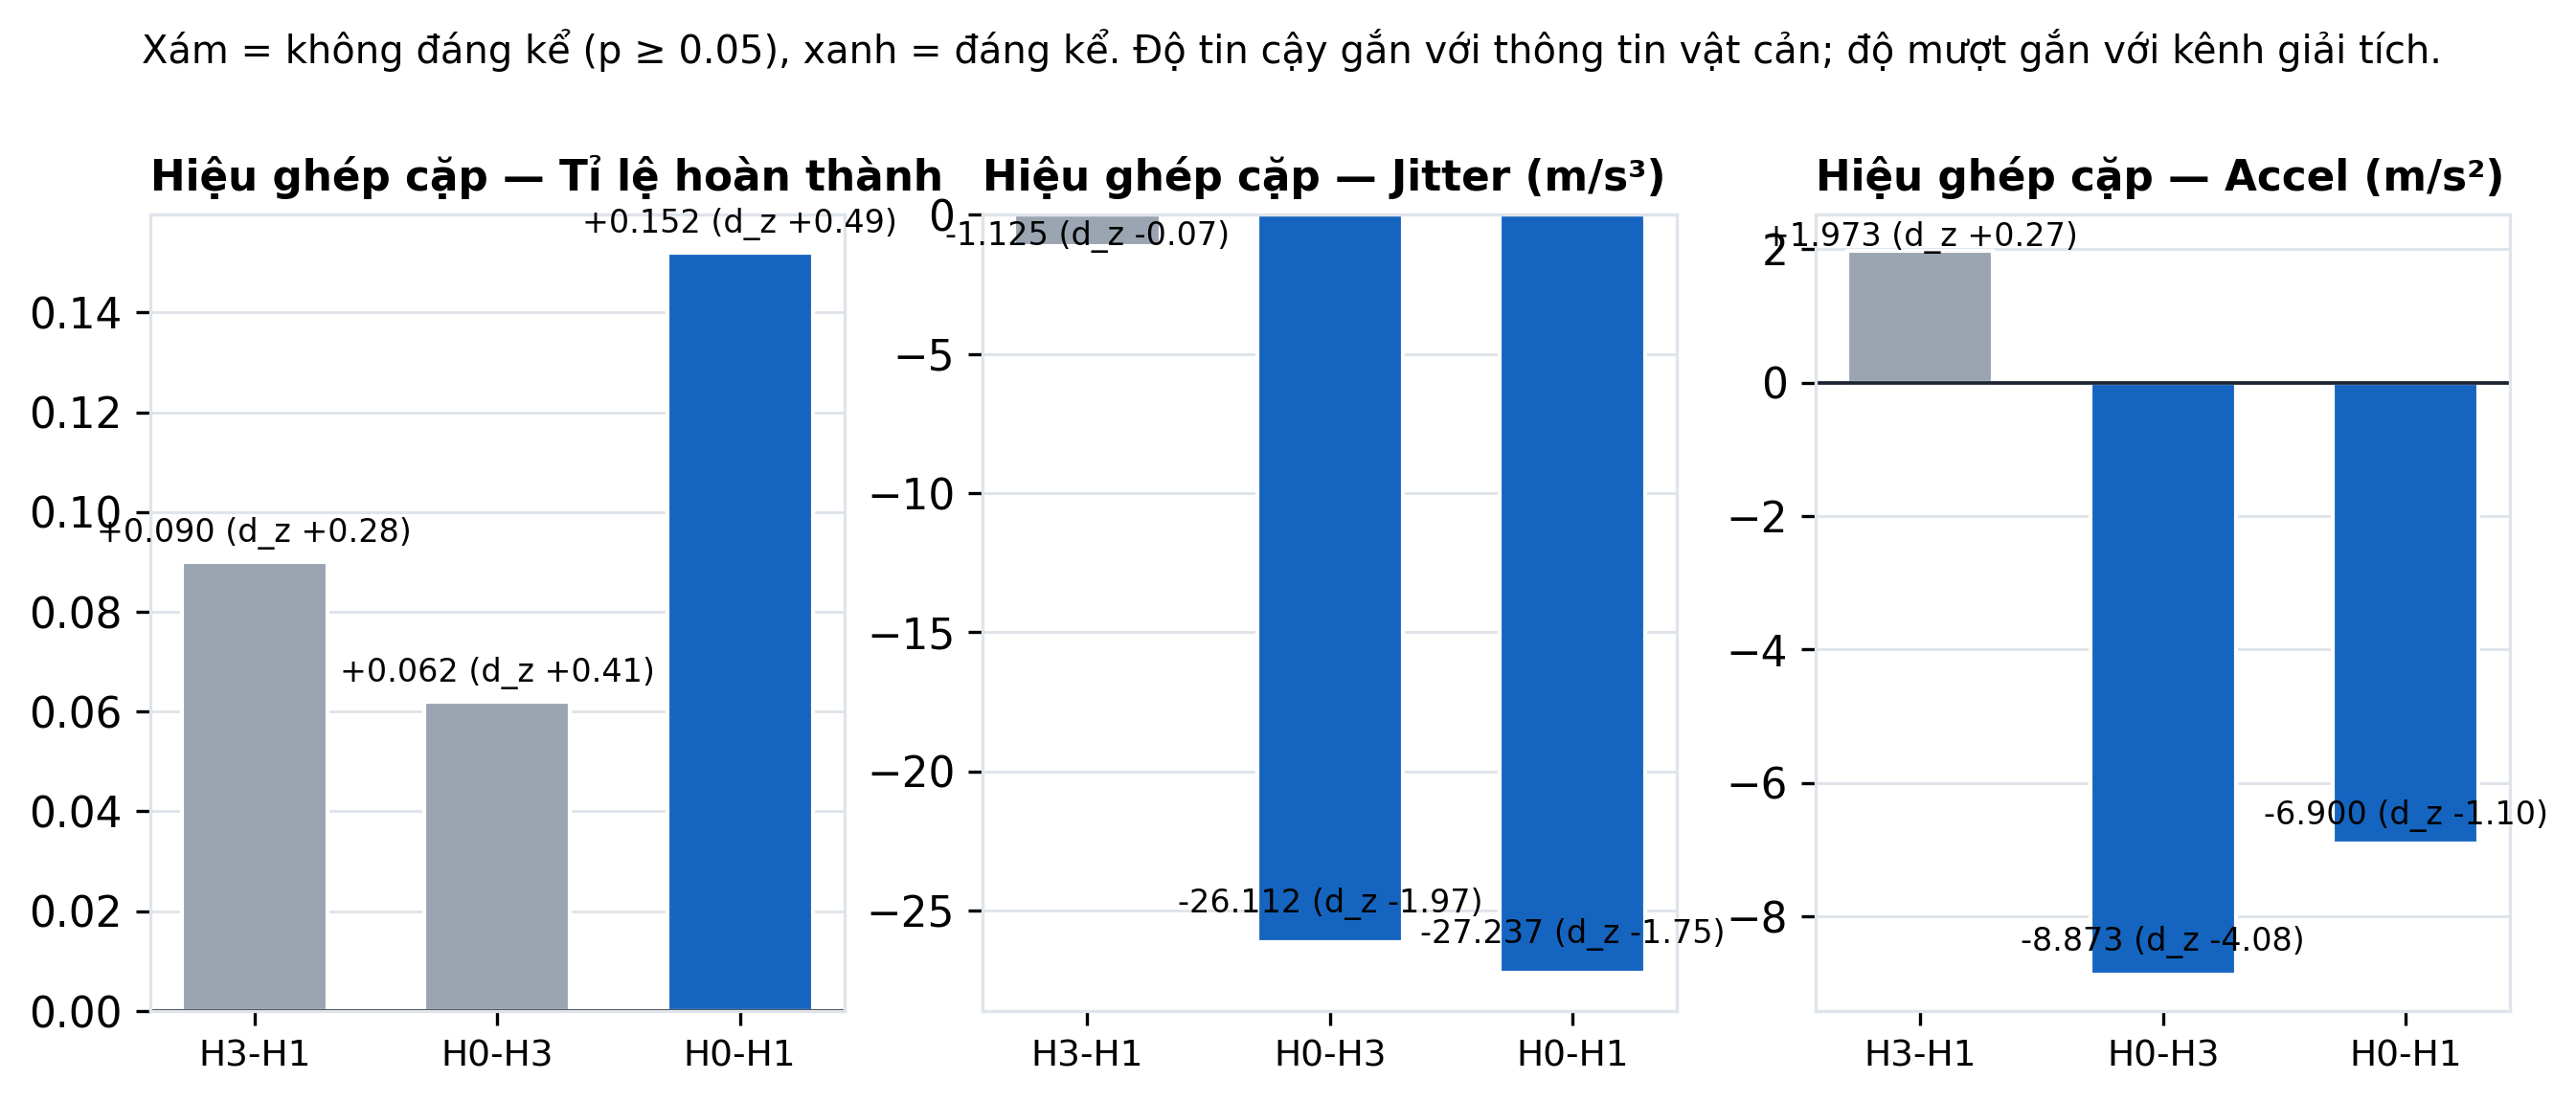
\includegraphics[width=0.93\textwidth]{figures/fig_disentanglement.png}
\caption{Decomposition of the hybrid advantage on corrected seeds. Grey bars are non-significant ($p\ge0.05$),
blue bars significant. Reliability gains attach to obstacle information in point estimate but reach significance
only in total; reduced sampled trajectory variation attaches to the analytical channel and is significant on its own.}
\label{fig:disentangle}
\end{figure*}
\subsection{Wind stress test on frozen policies}
Under $\texttt{wind\_scale}\in\{0,0.5,1,1.5,2\}$ (1000 rollouts per configuration per scale), H0 holds
100.0/100.0/100.0/99.5/98.6\% success with collisions as the only failure mode; H3 declines monotonically
96.9/96.1/93.8/92.6/91.5\%; H1 is flat and non-monotone (84.5/83.7/84.8/84.8/86.6\%), indicating that H1's deficit
is geometry- and control-driven rather than wind-driven. We therefore state graceful degradation up to twice the
training wind intensity for the frozen hybrid, and no robustness claim beyond the tested range.
\begin{table}[t]
\centering
\caption{Frozen-policy wind stress test: success per 1000 rollouts (collisions in parentheses).}
\label{tab:wind}
\begin{tabular}{lccccc}
\toprule
Config & 0.0 & 0.5 & 1.0 & 1.5 & 2.0\\
\midrule
H0 & 1000 (0) & 1000 (0) & 1000 (0) & 995 (5) & 986 (14)\\
H3 & 969 (31) & 961 (39) & 938 (62) & 926 (74) & 915 (85)\\
H1 & 845 (55) & 837 (50) & 848 (45) & 848 (49) & 866 (49)\\
\bottomrule
\end{tabular}
\end{table}
\subsection{APF sensitivity: distance basis dominates, $d_0$ does not}
Over 200 rollouts per setting, center-basis APF-only yields an identical 21/200 successes (172 collisions) for
$d_0=4,6,8,12$ m: the repulsive term never activates within $d_0$ of any box center along flown paths, so the
previously reported 5.5\% success measured a dead repulsion law rather than a property of potential-field
guidance. Surface-basis APF removes collisions entirely (0/200) and raises success to 88/200 ($d_0=4,6$) and
85/200 ($d_0=8,12$), with all remaining failures timeouts. APF-only therefore remains an insufficient planner
(stagnation), but its catastrophic collision rate was an implementation artifact; both facts are reported.
\begin{table}[t]
\centering
\caption{APF-only sensitivity, 200 rollouts per setting over the four training maps.}
\label{tab:sens}
\begin{tabular}{lcccc}
\toprule
Basis / $d_0$ (m) & 4 & 6 & 8 & 12\\
\midrule
center success & 21 & 21 & 21 & 21\\
center collision & 172 & 172 & 172 & 172\\
surface success & 88 & 88 & 85 & 85\\
surface collision & 0 & 0 & 0 & 0\\
surface timeout & 112 & 112 & 115 & 115\\
\bottomrule
\end{tabular}
\end{table}
\subsection{Held-out layouts}
On unseen layouts of the same families, H0 transfers at 250/250 (random, corridor, barrier), H3 at 203--250/250,
and H1 at 144--250/250. On the unseen mixed family all controllers collapse: H0 50/250, H3 17/250, H1 0/250,
every failure a collision, despite 233--250/250 on the training mixed map. The ordering H0 $>$ H3 $>$ H1 persists
on that family, but no generalization claim survives a 200/250 collision rate on one unseen layout family.
\begin{table}[t]
\centering
\caption{Held-out layouts: success per 250 rollouts (models frozen, same-layout training map).}
\label{tab:heldout}
\begin{tabular}{lcccc}
\toprule
Config & random & corridor & barrier & mixed\\
\midrule
H0 & 250 & 250 & 250 & 50\\
H3 & 203 & 250 & 222 & 17\\
H1 & 144 & 241 & 200 & 0\\
\bottomrule
\end{tabular}
\end{table}
\subsection{Blend sensitivity and action diagnostics}
Re-evaluating frozen H0 policies with constant $\lambda\in\{0.15,0.35,0.55\}$ gives 990/795/606 successes per
1000 versus 1000 under the adaptive schedule, with corridor success falling 250/246/172/0. Because training used
the adaptive schedule, this is deployment-time blend sensitivity, not a causal ablation. Step-level logging over
1000 H0 episodes shows $\|a^{\rm A2C}\|=1.458\pm0.132$, $\|a^{\rm APF}\|=0.0400\pm0.0000$ (exactly the attractive
gain: repulsion essentially never activates in successful flights), $\lambda=0.375\pm0.029$, cosine alignment
$0.545\pm0.054$, and per-step blended-action change $0.130\pm0.031$. These are mechanistic diagnostics: the
analytical channel acts as a small steady goal-directed bias whose distance-adaptive weighting, not its
repulsion, coincides with the hybrid's completion and variation profile.

\section{Discussion}
The matched-information baseline changes the interpretation of the hybrid's advantage without changing its sign.
Obstacle information accounts for most of the point-estimate reliability gap between hybrid and blind control,
yet neither information nor analytical channel reaches significance alone at $n=20$; only their sum does. The
variation result is the mirror image: it survives information matching (H0$-$H3 significant, H3$-$H1 null), so
the analytical channel's defensible contribution is damping of sampled trajectory variation, consistent with the
logged blend behavior. Two negative results bound the story: one unseen layout family collapses every
controller, and APF-only stagnates even with a correct distance basis. Remaining open items are a causal
fixed-$\lambda$ training ablation, matched-information held-out evaluation of H3 variants, surface-distance
guidance inside the hybrid, and any higher-fidelity or hardware validation.

\section{Threats to Validity}
H3's padded raw geometry and H0's center-distance APF input are different representations, so H0$-$H3 compares
analytical guidance under unequal geometric encodings; H3$-$H1 isolates information but not representation format.
Held-out evaluation supplies new geometry to H0/H3 channels and is transfer, not zero-shot generalization.
The wind sweep scales base and gust with one factor and is a stress test, not calibrated turbulence. Dynamics
remain point-mass with a 1-m altitude slab; acceleration and jerk are finite-difference trajectory-variation
diagnostics, not actuator or comfort measures. Success-only efficiency and clearance carry survivor composition
differences. Six-plus component tests are exploratory and uncorrected. Retraining is not bitwise reproducible;
archival analysis from the ledger is exact.

\section{Conclusion}
Adding a geometry-aware, APF-free baseline to a corrected-seed protocol separates what a hybrid A2C--APF
controller owes to obstacle information from what it owes to its analytical channel: most of the reliability
point-estimate, and essentially all of the statistically supported trajectory-variation benefit, respectively,
with the reliability components individually non-significant at 20 paired units. Frozen-policy stress tests show
graceful wind degradation to $2\times$ training intensity, transfer on three of four unseen layout families with
one family collapsing all controllers, and an APF-only baseline whose earlier failure was a dead center-distance
repulsion law. All null results are retained, and every claim is labelled with the evidence that supports it.

\bibliographystyle{IEEEtran}
\bibliography{references}
\end{document}
